\subsection*{Aufgabe 8}
Zwischen zwei Punkten befindet sich eine elektrische Leitung mit vier Schaltelementen S$_{1}$,
S$_{2}$, S$_{3}$ und S$_{4}$ (siehe Skizze).

\begin{center}
\begin{figure}[!htbp]
\fbox{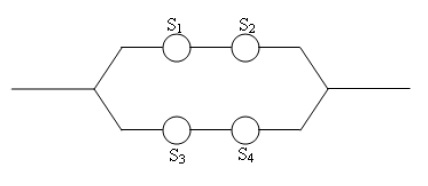
\includegraphics[width=0.8\textwidth,page=1]{chapters_AB/Grafiken_AB/AB_3_8.jpg}} 
\end{figure}
\end{center}

Die Leitung f�llt genau dann aus, wenn sowohl (mindestens) eines der beiden Elemente S$_{1}$, S$_{2}$ als auch (mindestens) eines der beiden Elemente S$_{3}$, S$_{4}$ ausf�llt. Nehmen Sie an, dass alle Ausf�lle unabh�ngig voneinander stattfinden! Machen Sie sich klar, was diese Annahme inhaltlich bedeutet!

\begin{enumerate}[leftmargin=0.8cm, label=\alph*)]
\item Mit welcher Wahrscheinlichkeit f�llt die Leitung aus, wenn die Ausfallwahrscheinlichkeiten der Schaltelemente (innerhalb eines bestimmten Zeitintervalls) alle identisch sind und jeweils 1\% betragen?
\item F�r die vier Schaltelemente stehen jeweils drei Ausf�hrungen A1, A2, A3 zur Auswahl
mit Preisen x$_{1}$ < x$_{2}$ < x$_{3}$ (x$_{1}$ = 1, x$_{2}$ = 2, x$_{3}$ = 10). Die Ausf�hrung Ai f�llt in einer
bestimmten Zeiteinheit mit Wahrscheinlichkeit pi aus (p$_{1}$ = 0,1, p$_{2}$ = 0,05, p$_{3}$ = 0,01).
Welches ist der niedrigstm�gliche Preis f�r die gesamte Anordnung, wenn 0,005 als
obere Schranke f�r die Ausfallwahrscheinlichkeit der gesamten Leitung vorgeschrieben
ist? Verwenden Sie Software zur L�sung der Aufgabe!
\end{enumerate}